% Stress test talk: a deck built to break identity, merging and pulling. Every frame carries
% something that is ambiguous on purpose (repeated titles, repeated text, repeated pictures,
% repeated cell values, repeated notes) or hard to index (astral characters, combining marks,
% NBSP, soft hyphens, RTL, CJK, a 400 character line, an empty item).
%
% Guards, as in tests/decks/sync/talk.tex (build.py resolves them per variant):
%   %<flag> line        the rest of the line only when the flag is set
%   %<!flag> line       the rest of the line only when the flag is not set
%   %<*flag> ... %</flag>, %<*!flag> ... %</!flag>   the same for blocks of lines
%
% Compiled with lualatex: the unicode frames need system fonts (Cambria Math, Microsoft YaHei,
% Times New Roman, Segoe UI Emoji), which only a unicode engine can load.
%<!fourthree>\documentclass[aspectratio=169]{beamer}
%<fourthree>\documentclass{beamer}
\usetheme{Madrid}
\setbeamertemplate{navigation symbols}{}
\setbeameroption{show notes}
\usepackage{amsmath,amssymb,booktabs,multirow}
\usepackage{fontspec}
\usepackage{graphicx}
\usepackage[absolute,overlay]{textpos}
\usepackage{tikz}
\usetikzlibrary{positioning,arrows.meta}
\newfontfamily\astralfont{Cambria Math}
\newfontfamily\cjkfont{Microsoft YaHei}
\newfontfamily\rtlfont{Times New Roman}
\newfontfamily\emojifont{Segoe UI Emoji}

% Every frame title goes through \T, so one flag renames all of them at once.
%<!retitleall>\newcommand{\T}[1]{#1}
%<retitleall>\newcommand{\T}[1]{#1 v2}

\title[Stress]{\T{A Deck Built to Break the Merge}}
\subtitle{Ambiguity, repetition and characters that do not fit in one code unit}
\author[B.~Builder]{Bea Builder}
\institute[Lab]{Laboratory of Hard Cases}
\date{September 2026}

\begin{document}

%<*!dropends>
\begin{frame}[label=title]
  \titlepage
\end{frame}

%</!dropends>
\begin{frame}[label=agenda]{\T{Agenda}}
  \begin{itemize}
    \item Slides that look alike
      \begin{itemize}
        \item twins one word apart
          \begin{itemize}
            \item the same paragraph three times
              \begin{description}
                \item[deepest] the same picture twice on one slide
              \end{description}
          \end{itemize}
      \end{itemize}
    \item Characters that break naive indexing
    \item Tables nobody wants to merge
  \end{itemize}
  \note{Set expectations: nothing here is meant to be pretty.}
\end{frame}

%<*!swaptwins>
\begin{frame}[label=twin-a]{\T{Twin slides}}
  \begin{itemize}
    \item The merge has to tell these two frames apart
    \item Only one word below is different
    \item This bullet is about identity, not about content
  \end{itemize}
  \note{Twin one. The next slide differs in a single word.}
\end{frame}

%</!swaptwins>
%<*insertframe>
\begin{frame}[label=between]{\T{Inserted between the twins}}
  \begin{itemize}
    \item A frame added exactly where identity is hardest
    \item Its neighbours are one word apart
  \end{itemize}
\end{frame}

%</insertframe>
\begin{frame}[label=twin-b]{\T{Twin slides}}
  \begin{itemize}
    \item The merge has to tell these two frames apart
    \item Only one word above is different
    \item This bullet is about identity, not about content
  \end{itemize}
  \note{Twin two. The previous slide differs in a single word.}
\end{frame}

%<*swaptwins>
\begin{frame}[label=twin-a]{\T{Twin slides}}
  \begin{itemize}
    \item The merge has to tell these two frames apart
    \item Only one word below is different
    \item This bullet is about identity, not about content
  \end{itemize}
  \note{Twin one. The next slide differs in a single word.}
\end{frame}

%</swaptwins>
\begin{frame}[label=echo-one]{\T{Echo, first time}}
  Nothing in this paragraph says which slide it is on, which is the whole point of repeating it.

  \medskip
  Context for the first echo: the deck was converted once.
  \note{Echo one of three.}
\end{frame}

\begin{frame}[label=echo-two]{\T{Echo, second time}}
  Nothing in this paragraph says which slide it is on, which is the whole point of repeating it.

  \medskip
  Context for the second echo: the deck was edited by hand.
  \note{Echo two of three.}
\end{frame}

\begin{frame}[label=echo-three]{\T{Echo, third time}}
  Nothing in this paragraph says which slide it is on, which is the whole point of repeating it.

  \medskip
  Context for the third echo: the source changed again.
  \note{Echo three of three.}
\end{frame}

\begin{frame}[label=astral]{\T{Characters outside the BMP}}
  \begin{itemize}
    \item Mathematical letters: {\astralfont 𝐀𝔻𝕏} count as two code units each
    \item An emoji: {\emojifont 😀} and a plain symbol: {\emojifont ☺}
    \item Combining marks: \={x} and \'{e} and \v{s} stay one grapheme
  \end{itemize}
  \note{Every index in the merge is a UTF-16 index.}
\end{frame}

\begin{frame}[label=scripts]{\T{Other scripts and invisible characters}}
  \begin{itemize}
    \item Chinese: {\cjkfont 同步测试幻灯片}
    \item Hebrew, right to left: {\rtlfont שלום עולם}
    \item A no-break space holds 12~kg together
    \item A soft hyphen hides inside super\-cali\-fragilistic\-expialidocious
  \end{itemize}
  \note{Every index in the merge is a UTF-16 index.}
\end{frame}

\begin{frame}[label=longline]{\T{One very long line}}
  The following sentence is deliberately four hundred characters long so that a word level merge
  has to walk a long way before it finds the one word that changed, and so that the converter has
  to wrap it into several lines of one paragraph, which is exactly the case where an off by one in
  a character index is impossible to see by eye and very easy to ship.
  \note{Four hundred characters, one paragraph.}
\end{frame}

\begin{frame}[label=gaps]{\T{Gaps and ragged ends}}
  \begin{itemize}
    \item A list with an empty item follows
    \item[]
    \item And the slide ends without a full stop
  \end{itemize}
  A closing paragraph with no terminator
  \note{An empty item and an unterminated line.}
\end{frame}

\begin{frame}[label=bigtable]{\T{Twenty rows}}
  \centering
  \tiny
  \begin{tabular}{lrl}
    \toprule
    Case & Time & Verdict \\
    \midrule
%<!everyrow>    Alpha & 1.0 s & kept \\
%<everyrow>    Alpha & 1.1 s & kept \\
%<!everyrow>    Beta & 1.0 s & kept \\
%<everyrow>    Beta & 1.2 s & kept \\
%<!everyrow>    Gamma & 1.0 s & kept \\
%<everyrow>    Gamma & 1.3 s & kept \\
%<!everyrow>    Delta & 1.0 s & kept \\
%<everyrow>    Delta & 1.4 s & kept \\
%<!everyrow>    Epsilon & 1.0 s & kept \\
%<everyrow>    Epsilon & 1.5 s & kept \\
%<!everyrow>    Zeta & 1.0 s & kept \\
%<everyrow>    Zeta & 1.6 s & kept \\
%<!everyrow>    Eta & 1.0 s & kept \\
%<everyrow>    Eta & 1.7 s & kept \\
%<!everyrow>    Theta & 1.0 s & kept \\
%<everyrow>    Theta & 1.8 s & kept \\
%<!everyrow>    Iota & 1.0 s & kept \\
%<everyrow>    Iota & 1.9 s & kept \\
%<!everyrow>    Kappa & 1.0 s & kept \\
%<everyrow>    Kappa & 2.0 s & kept \\
%<!everyrow>    Lambda & 1.0 s & kept \\
%<everyrow>    Lambda & 2.1 s & kept \\
%<!everyrow>    Mu & 1.0 s & kept \\
%<everyrow>    Mu & 2.2 s & kept \\
%<!everyrow>    Nu & 1.0 s & kept \\
%<everyrow>    Nu & 2.3 s & kept \\
%<!everyrow>    Xi & 1.0 s & kept \\
%<everyrow>    Xi & 2.4 s & kept \\
%<!everyrow>    Omicron & 1.0 s & kept \\
%<everyrow>    Omicron & 2.5 s & kept \\
%<!everyrow>    Pi & 1.0 s & kept \\
%<everyrow>    Pi & 2.6 s & kept \\
%<!everyrow>    Rho & 1.0 s & kept \\
%<everyrow>    Rho & 2.7 s & kept \\
%<!everyrow>    Sigma & 1.0 s & kept \\
%<everyrow>    Sigma & 2.8 s & kept \\
%<!everyrow>    Tau & 1.0 s & kept \\
%<everyrow>    Tau & 2.9 s & kept \\
%<!everyrow>    Upsilon & 1.0 s & kept \\
%<everyrow>    Upsilon & 3.0 s & kept \\
    \bottomrule
  \end{tabular}

  \medskip
  {\footnotesize Twenty rows, one verdict.}
  \note{Every row says the same thing on purpose.}
\end{frame}

\begin{frame}[label=widetable]{\T{Ten columns}}
  \centering
  \tiny
  \begin{tabular}{lrrrrrrrrr}
    \toprule
    Run & C1 & C2 & C3 & C4 & C5 & C6 & C7 & C8 & C9 \\
    \midrule
    First & 7 & 7 & 7 & 7 & 7 & 7 & 7 & 7 & 7 \\
    Second & 7 & 8 & 7 & 8 & 7 & 8 & 7 & 8 & 7 \\
    Third & 7 & 7 & 7 & 7 & 7 & 7 & 7 & 7 & 7 \\
    \bottomrule
  \end{tabular}
  \note{Ten columns of sevens.}
\end{frame}

\begin{frame}[label=merged]{\T{Merged cells}}
  \centering
  \small
  \begin{tabular}{lcc}
    \toprule
    Phase & \multicolumn{2}{c}{Measured} \\
    \cmidrule(lr){2-3}
    & Before & After \\
    \midrule
    \multirow{2}{*}{Planning} & 7 & 7 \\
    & 7 & 8 \\
    Writing & 7 & 7 \\
    \bottomrule
  \end{tabular}
  \note{One cell spans two columns, another two rows.}
\end{frame}

\begin{frame}[label=columns]{\T{Two columns of text}}
  \begin{columns}[t]
    \column{0.47\textwidth}
    The left column argues that identity must come from labels, because titles repeat and
    positions move.
    \column{0.47\textwidth}
    The right column argues the same thing in different words, so that a similarity score alone
    cannot decide which column is which.
  \end{columns}
  \note{Two columns that argue the same thing.}
\end{frame}

\begin{frame}[label=blockcol]{\T{A block inside a column}}
  \begin{columns}[t]
    \column{0.5\textwidth}
%<!rewriteblock>    \begin{block}{Rule}
%<rewriteblock>    \begin{block}{Rule, restated}
%<!rewriteblock>      Deck edits win, and the source is told so in the report.
%<rewriteblock>      The deck always wins, and the report explains why.
    \end{block}
    \column{0.45\textwidth}
    A block that lives in a column has to keep its panel, its title bar and its shadow when the
    group is rebuilt.
  \end{columns}
  \note{The block has to survive being rebuilt.}
\end{frame}

\begin{frame}[label=boxes]{\T{Twelve text boxes}}
  \begin{textblock*}{2.2cm}(0.8cm,2.4cm) Box one \end{textblock*}
  \begin{textblock*}{2.2cm}(3.4cm,2.4cm) Box two \end{textblock*}
  \begin{textblock*}{2.2cm}(6.0cm,2.4cm) Box three \end{textblock*}
  \begin{textblock*}{2.2cm}(8.6cm,2.4cm) Box four \end{textblock*}
  \begin{textblock*}{2.2cm}(0.8cm,3.6cm) Box five \end{textblock*}
  \begin{textblock*}{2.2cm}(3.4cm,3.6cm) Box six \end{textblock*}
  \begin{textblock*}{2.2cm}(6.0cm,3.6cm) Box seven \end{textblock*}
  \begin{textblock*}{2.2cm}(8.6cm,3.6cm) Box eight \end{textblock*}
  \begin{textblock*}{2.2cm}(0.8cm,4.8cm) Box nine \end{textblock*}
  \begin{textblock*}{2.2cm}(3.4cm,4.8cm) Box ten \end{textblock*}
  \begin{textblock*}{2.2cm}(6.0cm,4.8cm) Box eleven \end{textblock*}
  \begin{textblock*}{2.2cm}(8.6cm,4.8cm) Box twelve \end{textblock*}
  \note{Twelve boxes, twelve element keys.}
\end{frame}

\begin{frame}[label=formulas]{\T{Formulas side by side}}
  The line holds $\frac{a}{b}$ $\sqrt{x+1}$ $\sum_{i=1}^{n} x_i$ with nothing between them, so
  three pictures have to share the gaps of one line of prose.

  \medskip
  A second line puts $\hat{\beta}_{t}^{(k)}$ right after $\frac{\partial L}{\partial \theta}$ again.
  \note{Three holes in one line of prose.}
\end{frame}

\begin{frame}[label=steps]{\T{Steps that appear one by one}}
  \begin{itemize}
    \item Read the base
    \pause
    \item Convert the source
    \pause
    \item Merge and write
  \end{itemize}
  \note{The deck keeps the last step only.}
\end{frame}

\begin{frame}[label=alternatives]{\T{Alternatives on one frame}}
  \only<1>{The first version of this sentence is never kept.}
  \only<2>{The second version of this sentence is the one that survives.}
  \note{Only the last step reaches the deck.}
\end{frame}

\begin{frame}[label=figcaption]{\T{A figure with a caption}}
  \centering
  \begin{figure}
    \includegraphics[width=3cm]{figures/wave.png}
    \caption{A caption that names the picture it sits under}
  \end{figure}
  \note{The caption belongs to the picture.}
\end{frame}

\begin{frame}[label=twinpics]{\T{Two identical pictures}}
  \centering
  \includegraphics[width=3cm]{figures/dot.png}
  \hspace{2cm}
%<!swappicture>  \includegraphics[width=3cm]{figures/dot.png}
%<swappicture>  \includegraphics[width=3cm]{figures/wave.png}

  \medskip
  The same file twice: only their boxes tell them apart.
  \note{Two pictures with the same bytes.}
\end{frame}

\begin{frame}[label=picagain]{\T{The same picture again}}
  \centering
  \includegraphics[width=3cm]{figures/dot.png}

  \medskip
  And once more, on another slide.
  \note{The same bytes again, one slide later.}
\end{frame}

\begin{frame}[label=fullpage,plain]
  \begin{tikzpicture}[remember picture,overlay]
    \node at (current page.center) {\includegraphics[width=\paperwidth]{figures/wide.png}};
  \end{tikzpicture}
\end{frame}

\begin{frame}[label=onlypic]
  \centering
  \vfill
  \includegraphics[width=4cm]{figures/wave.png}
  \vfill
\end{frame}

\begin{frame}[label=results-a]{\T{Results}}
  \centering
  \small
  \begin{tabular}{lrr}
    \toprule
    Scenario & Kept & Time \\
    \midrule
    Disjoint & 100\% & 7 s \\
    Same element & 100\% & 7 s \\
    Conflicts & 92\% & 7 s \\
    \bottomrule
  \end{tabular}
  \note{Three slides are called Results. That is the test.}
\end{frame}

\begin{frame}[label=results-b]{\T{Results}}
  \begin{itemize}
    \item Every deck edit survived
    \item Every source change landed
  \end{itemize}
  \note{Three slides are called Results. That is the test.}
\end{frame}

\begin{frame}{\T{Results}}
  This third slide called Results has no label at all, so only its content can identify it.
  \note{Three slides are called Results. That is the test.}
\end{frame}

\begin{frame}[label=notes-a]{\T{Notes, one}}
  A slide whose speaker notes are shared with another slide.
%<!notesedit>  \note{Remember to slow down here; the audience needs a moment.}
%<notesedit>  \note{Slow right down here; give the audience a moment to catch up.}
\end{frame}

\begin{frame}[label=notes-b]{\T{Notes, two}}
  A second slide whose speaker notes are word for word the same.
  \note{Remember to slow down here; the audience needs a moment.}
\end{frame}

\begin{frame}[label=diagram]{\T{A small diagram}}
  \centering
  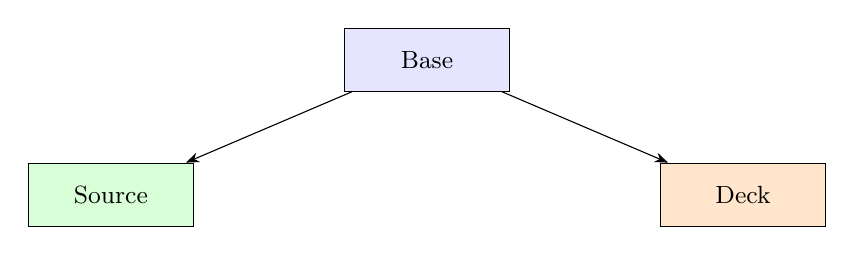
\begin{tikzpicture}[node distance=0.9cm and 1.9cm, every node/.style={font=\small}]
    \node[draw, fill=blue!10, minimum width=2.1cm, minimum height=0.8cm] (base) {Base};
    \node[draw, fill=green!15, minimum width=2.1cm, minimum height=0.8cm, below left=of base] (ours) {Source};
    \node[draw, fill=orange!20, minimum width=2.1cm, minimum height=0.8cm, below right=of base] (theirs) {Deck};
    \draw[-{Stealth}] (base) -- (ours);
    \draw[-{Stealth}] (base) -- (theirs);
  \end{tikzpicture}
  \note{Nodes and edges become shapes, not a picture.}
\end{frame}

\begin{frame}[label=displaymath]{\T{Display mathematics}}
  \[
    \mathcal{L}(\theta) = \sum_{i=1}^{n} \bigl\lVert y_i - f_\theta(x_i) \bigr\rVert^2
    + \lambda \int_0^1 \frac{\partial^2 f}{\partial x^2}\,dx
  \]
  The equation stays a picture; the sentence around it does not.
  \note{Display maths never comes back as text.}
\end{frame}

\begin{frame}[label=code,fragile]{\T{A code block}}
\begin{verbatim}
def merge(base, ours, theirs):
    if ours == base:
        return theirs
    return diff3(base, ours, theirs)
\end{verbatim}
\end{frame}

\begin{frame}[label=links]{\T{Links in the text}}
  An external link to \href{https://example.org/sync}{the sync documentation} and an internal one
  back to \hyperlink{agenda}{the agenda}.
  \note{One link leaves the deck, one stays inside it.}
\end{frame}

\begin{frame}[label=numbers]{\T{Numbered steps}}
  \begin{enumerate}
    \item Read the base snapshot
    \item Convert the new source
    \item Read the live deck
    \item Merge and write
  \end{enumerate}
\end{frame}

\begin{frame}[label=description]{\T{Description list}}
  \begin{description}
    \item[base] what the converter produced last time
    \item[ours] the conversion of the changed source
    \item[theirs] the deck as it is now
  \end{description}
  \note{Hanging labels become a tab.}
\end{frame}

\begin{frame}[label=quote]{\T{A quotation}}
  \begin{quote}
    Deck edits win; the source is told what it could not apply.
  \end{quote}
  The sentence above is quoted twice in this deck on purpose.
\end{frame}

\begin{frame}[label=emphasis]{\T{Emphasis of every kind}}
  \begin{itemize}
    \item \textbf{Bold}, \emph{italic}, \texttt{monospace} and \alert{alerted} words
    \item \textcolor{red!70!black}{Coloured} words next to \underline{underlined} ones
  \end{itemize}
\end{frame}

\begin{frame}[label=deep]{\T{Deep nesting again}}
  \begin{itemize}
    \item First level
      \begin{itemize}
        \item Second level
          \begin{itemize}
            \item Third level
              \begin{description}
                \item[fourth] Fourth level
              \end{description}
          \end{itemize}
      \end{itemize}
  \end{itemize}
  \note{Four levels is as deep as beamer goes.}
\end{frame}

%<!movelabel>\begin{frame}[label=mobile]{\T{Moving labels}}
%<movelabel>\begin{frame}{\T{Moving labels}}
  The label on this frame moves to the next one in one of the variants.
\end{frame}

%<!movelabel>\begin{frame}[label=arriving]{\T{Arriving labels}}
%<movelabel>\begin{frame}[label=mobile]{\T{Arriving labels}}
  This frame is where that label arrives.
\end{frame}

%<!nolabel>\begin{frame}[label=vanishing]{\T{Disappearing label}}
%<nolabel>\begin{frame}{\T{Disappearing label}}
  This frame loses its label in one of the variants, so its key falls back to its title.
\end{frame}

\begin{frame}[label=footnotes]{\T{Footnotes and small print}}
  A claim that needs a footnote.\footnote{The footnote is small print at the bottom.}
\end{frame}

\begin{frame}[label=repeatcells]{\T{Cells that repeat a value}}
  \centering
  \small
  \begin{tabular}{llll}
    \toprule
    Slide & Text & Style & Geometry \\
    \midrule
%<!everyrow>    One & same & same & same \\
%<everyrow>    One & same & same & moved \\
%<!everyrow>    Two & same & same & same \\
%<everyrow>    Two & same & same & moved \\
%<!everyrow>    Three & same & same & same \\
%<everyrow>    Three & same & same & moved \\
%<!everyrow>    Four & same & same & same \\
%<everyrow>    Four & same & same & moved \\
%<!everyrow>    Five & same & same & same \\
%<everyrow>    Five & same & same & moved \\
%<!everyrow>    Six & same & same & same \\
%<everyrow>    Six & same & same & moved \\
    \bottomrule
  \end{tabular}
  \note{Six rows that say the same thing in the same words.}
\end{frame}

\begin{frame}[label=whitespace]{\T{Whitespace only}}
%<!whitespace>  A paragraph whose words never change, only the spaces between them in the source.
%<whitespace>  A   paragraph  whose words never  change,   only the spaces between them in the source.

  \medskip
  A second paragraph, kept as a witness.
\end{frame}

\begin{frame}[label=quote-again]{\T{The quotation, again}}
  \begin{quote}
    Deck edits win; the source is told what it could not apply.
  \end{quote}
  The same sentence as before, on a different slide.
\end{frame}

\begin{frame}[label=backup]{\T{Backup material}}
  \begin{itemize}
%<!rewritebullets>    \item Timings are measured on the stress deck itself
%<rewritebullets>    \item Every timing below comes from this deck and no other
%<!rewritebullets>    \item Nothing here is shown in the talk
%<rewritebullets>    \item None of it is shown while the talk is running
%<!rewritebullets>    \item The numbers are rounded to whole seconds
%<rewritebullets>    \item Seconds are rounded, milliseconds are dropped
  \end{itemize}
  \note{Skip unless asked.}
\end{frame}

%<*!dropends>
\begin{frame}[label=summary]{\T{Takeaways}}
  \begin{itemize}
    \item Labels decide identity; titles and text never do
    \item Every index is a UTF-16 index
    \item Nothing is lost, even when everything is ambiguous
  \end{itemize}
  \note{Close on the rule: never lose data.}
\end{frame}

%</!dropends>
\end{document}
